\chapter{Custom Parts}

\textbf{Author: Fabian Kleinrad} 

This chapter is going to take a look at the practical side of the autumn project. When working with hardware there is the inevitable need for parts fit for the underling application. In case of autumn, with the Matrice 100 being in the center of the project the need arises to design and manufacture parts in order to make the hardware portion in autumn come together without any complication and potential weak points in the final product.

\section{Reasons}

The goal of the autumn project being as innovative and unique in terms of methods used in the realization of the project, parts needed are either not readily available or not compliant with the budget. Another difficulty are parts too specific for there to be any commercially available. Therefor to guaranty the reusability and reliability of the final product, methods to design and produce parts specifically tailored to the needs in the autumn project have to be utilized.

\subsection{Camera Mount}

Autumn conquers the problem of mapping an environment with the use of a drone. Therefore it is necessary to attach the camera used to capture the surrounding to the drone that allows it to move through that space. In case of autumn the camera being used is a ZED2i, which needs to be securely attached to an Matrice 100. Additionally to the cost factor and accompanied risk of damaging the hardware in use, the positioning and angle are important properties to consider. For that reason a commercial solution is precluded.

\subsubsection{First approach}

When working with the principle of fast prototyping, the drawback of first approaches being incomplete is inherit. Following this principle lead to attaching the ZED2i to the Matrice 100 with the help of zip ties. Rational for this decision being the reliability and strength of zip ties which allowed the camera to be secured tightly. This was important because of the need to test segments of the autumn project, worked on separately and isolated from one another. With taking simple and easy to realize steps it enables the project to progress more smoothly and without the need for other sub-areas to be set on hold because of long tedious planing and manufacturing periods of parts like an custom camera mount for a drone.

\subsubsection{Problems without a Mount}

After a period of testing with a prototype problems arise with the need of correction. In case of an, what most people consider a work-around rather than a solution to the problem of mounting a camera, they can be, in case of this application, divided in two categories.
The first aspect to consider when mounting a camera to a drone is its field of view. With UAVs hovering above ground an angle is needed in order to be able to capture details close to the ground.  

\begin{figure}[h]
	\centering
	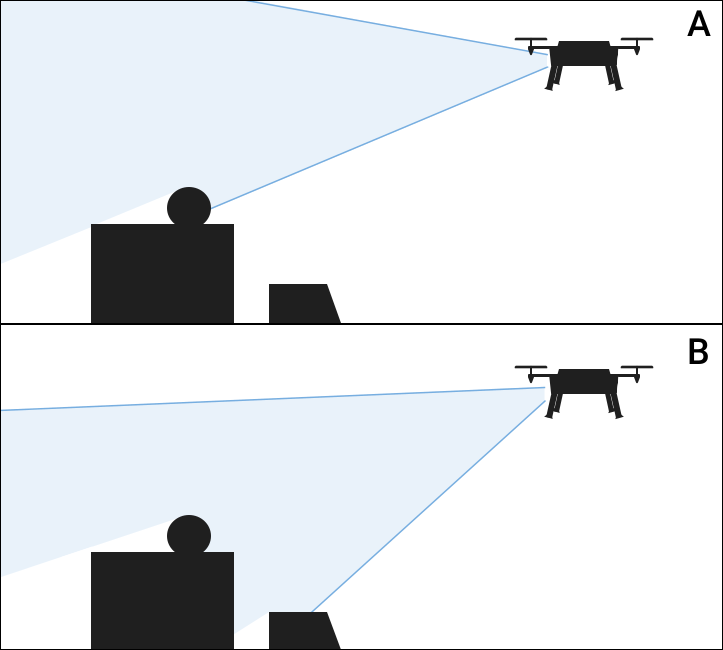
\includegraphics[width=0.7\linewidth]{img/FieldOfView}
	\caption{Depiction of the FOV for cameras mounted at different angles on a drone.\newline A: camera mounted vertically, B: camera mounted with a downward pointing angle.}
	\label{fig:custom_parts_FOV}
\end{figure}

\subsubsection{How the mount was made}

\section{CAD Software}

\subsubsection{Fusion 360}

\section{Manufacturing Process}

\subsection{Methods}

\section{3D Printing}

\subsection{FDM Printing}

\subsection{SLA Printing}